%%%%%%%%%%%%%%%%%%%%%%%%%%%%%%%%%%%%%%%%%%%%%%%%%%%%%%%%%%%%%%%%%%%%%%%%
% Preamble
%%%%%%%%%%%%%%%%%%%%%%%%%%%%%%%%%%%%%%%%%%%%%%%%%%%%%%%%%%%%%%%%%%%%%%%%
\documentclass[11pt]{article}
%
% Packages and other includes
% Pagination
\usepackage[letterpaper, margin=1in]{geometry}
\usepackage{emptypage}
%
% Fonts
\usepackage[T1]{fontenc} % best for Western European languages
\usepackage{lmodern} % Latin Modern instead of CM
\usepackage{textcomp} % required to get special symbols
%
% Math
\usepackage{amsmath, amssymb}
\usepackage{braket}
%
% Graphics, floats, tables
\usepackage{graphicx, color, float, array}
%
% Hyperlinks
\usepackage{hyperref}
%
%
% Definitions and settings
% Paragraph indent and spacing
\setlength{\parskip}{0.4\baselineskip}
\setlength{\parindent}{0in}
%
%
% Title, authors, date
\title{\textbf{Worksheet 2}}
\date{\vspace{-2em}January 11, 2022}
%
%
%%%%%%%%%%%%%%%%%%%%%%%%%%%%%%%%%%%%%%%%%%%%%%%%%%%%%%%%%%%%%%%%%%%%%%%%
% Main document
%%%%%%%%%%%%%%%%%%%%%%%%%%%%%%%%%%%%%%%%%%%%%%%%%%%%%%%%%%%%%%%%%%%%%%%%
%

\begin{document}

\maketitle

Weekly homework assignments are posted approximately one week prior to the
due date. Collaborations are encouraged and students must report all collaborators
in writing on each assignment. All external sources (websites, books) must be
properly cited. Additional problems are listed at the end of each assignment.
This week's assignment is due \textit{Tuesday, Jan 18th at 10:00am.}

\textbf{Ideal Gas Law}

1. (2 pts) What\ is the density (in g/L) of chloroform, CHCl$_3$, vapor at
$2.00\times 10^2\text{Torr}$ and $298\text{K}$. Report to 3 significant figures.

\vspace{1.5in}

2. (2 pts) A compound used in the manufacture of Saran is $24.7\%$ C, $2.10\%$ H, and
$73.2\%$ Cl by mass. The storage of $3.557\text{g}$ of the gaseous compound in
a $755$-mL vessel at $0^\circ\text{C}$ results in a pressure of $1.10\text{atm}$.
What is the molecular formula of the compound? Report to 3 significant figures.

% C2H2Cl2

\vspace{1.5in}

3. (2 pts) A vessel of volume $22.4\text{L}$ contains $2.00$ mol H$_2$(g) and $1.00$ mol
N$_2$(g) at $273.15\text{K}$. Calculate the partial pressures and the total pressure.
Report to 3 significant figures.

\vspace{1.7in}

4. (6 pts) A flask of volume 5.00L is evacuated and 43.78g of solid dinitrogen tetroxide,
N$_2$O$_4$, is introduced at $-196^\circ\text{C}$. The sample is then warmed to
$25^\circ\text{C}$, during which time the N$_2$O$_4$ vaporizes and some of it dissociates
to form brown NO$_2$ gas. The pressure slowly increases until it stabilizes at 2.96atm.
Report to 3 significant figures.

(a) Write a balanced equation for the reaction.

(b) If the gas in the flask at $25^\circ\text{C}$ were all N$_2$O$_4$, what would the pressure
be?

(c) If all the gas in the flask converted into NO$_2$, what would the pressure be?

(d) What are the mole fractions of N$_2$O$_4$ and NO$_2$ once the pressure stabilizes at
2.96atm?

\pagebreak

5. (8 pts) \textbf{Barometric Formula} The barometric formula is a model that predicts the
air pressure depending on the altitude. This formula assumes ideal gas conditions at constant
temperature T. Use the following steps to derive the barometric formula.

(a) Draw a free body diagram for a volume of air at some altitude. Define all variables. \textit{Hint:}
To get started, an illustration below is a volume of air defined by area (A) and height (dh).
Set up your axis system and draw all forces acting on the air.
\begin{center}
  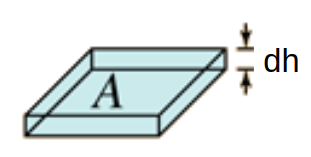
\includegraphics[scale=0.3]{air_vol.png}
\end{center}

(b) Based on the axis system, write an equation involving all forces acting on the air.
\textit{Hint:} The net force equals zero.

(c) Invoke the ideal gas law to replace variables in terms of molar mass, pressure,
temperature, and volume. Solve for pressure.

(d) The expression in (c) is a first order homogeneous linear differential equation and
has the form,
\begin{equation}
  \frac{dy}{dt} = -p(t)y.
\end{equation}
The solution can be determined via integration and has the form,
\begin{equation}
  y = Ce^{P(t)}
\end{equation}
where $P(t)$ is the antiderivative of $-p(t)$ and $C$ is a constant. Solve the differential
equation in (c).

(e) Mount Everest is Earth's highest mountain at 29,032 feet (8,848 meters). Each year,
approximately 1000 people hike Mount Everest. Use the expression in (d), estimate the
barometric pressure at the summit where the temperature is $-9^\circ\text{C}$.

%A hiker brings a mercury
%barometer to measure the height of Mount Everest. At the summit, the hiker reports the
%barometric pressure to be 253.0 Torr at $-9^\circ\text{C}$. Use the derived barometric
%formula to approximate the height of Mount Everest. Report to 4 significant figures.

% Deriving the Barometric Formula online
%
% https://www.youtube.com/watch?v=anAMD_KeB0s

\pagebreak

\textbf{First Law of Thermodynamics}

6. (4 pts) Calculate the work for each of the following processes beginning with a gas
sample in a piston assembly with $T=305\text{K}$, $P=1.79\text{atm}$, and
$V=52.9\text{L}$ by two different pathways. Report to 3 significant figures.

(a) Isothermal, reversible expansion to a final volume of $6.52\text{L}$.

(b) Irreversible expansion against a constant external pressure of $1.00\text{atm}$
to a final volume of $6.52\text{L}$.

\vfill
\textbf{Optional Additional Problems:} Ch. 10 - odd problems 95 - 117

\end{document}
